\chapter{How Active Directory Works}
Active Directory was first released with Windows Server 2000. Its primary function is to provide authentication, authorization, identity and access management, and directory services to users on a Windows-based network.
\begin{itemize}
    \item Authentication is the process where Active Directory verifies a user's credentials (username and password). The user credentials are stored in the Active Directory database (\texttt{ntds.dit}).
    \item Authorization is the process that grants or denies a user the ability to do something such as edit a file or access an application.
\end{itemize}

Since its release, Microsoft has added additional services to Active Directory. The topic of Active Directory can be quite complex as there are many components that are always in motion. Just remember that its core function is to authenticate and authorize users to use network resources.

Even though there has been a big push to move everything to the cloud, Active Directory is still used by most medium to large organizations. Many organizations use Microsoft Office 365 and cloud services and operate in a \textit{hybrid mode.} This means that the local Active Directory is synced with the cloud to provide seamless authentication to Office 365 resources, such as email.

To better understand how Active Directory works, let us look at some examples. These examples provide a high-level overview of how Active Directory works.

\subsection{Example 1: Authenticate Users}
Sam was recently hired as an accountant for Active Directory Pro. The IT administrator creates an account for Sam in Active Directory Users and Computers (ADUC). The account is unique to Sam and contains personal details such as first name, last name, office location, phone number, email address, etc. Sam is provided with a username and password so that she can log into the company network.
\begin{enumerate}
    \item Sam logs into her laptop with the username and password provided by the IT department.
    \item The logon request goes to the Active Directory Domain Controller (DC) or Authentication Server (AS) (depending on configuration) to verify and validate Sam's credentials.
    \item The DC or AS searches for Sam's account in the \texttt{ntds.dit} database. If the credentials match, Sam will be granted access. If not, she will be denied.
    \item If credential verification and validation are successful, Sam will be logged on to her laptop and will be authenticated against the domain.
\end{enumerate}
\begin{figure}
    \centering
    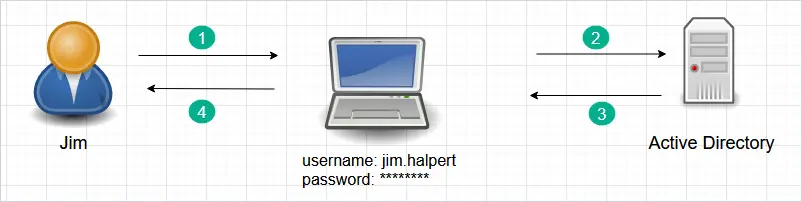
\includegraphics[width=0.75\linewidth]{domauth.png}
    \caption{Enter Caption}
    \label{fig:placeholder}
\end{figure}

\subsection{Example 2: Authorize User (Grant of Deny Permissions}
In this example, the Active Directory server will authorize access to network resources.
\begin{enumerate}
    \item Sam logs into her computer using the username and password provided and wants to access her email, a contract file, and the accounting database server.
    \item These network resources check with the DC or AS to see if Sam's account is authorized for access.
    \item The DC or AS then verify Sam's account and either grants the account access or not.
    \item Sam's account is granted access, and she can now check her email, modify the contract file, and work on the database server.
    \begin{figure}
        \centering
        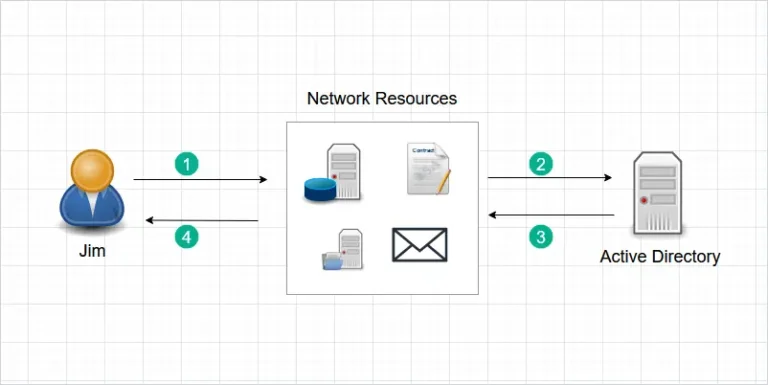
\includegraphics[width=0.75\linewidth]{authorization.png}
        \caption{Enter Caption}
        \label{fig:placeholder}
    \end{figure}
\end{enumerate}

\subsection{Example 3: Authorize and Deny User Access}
In this last example, we will look at another user that has mixed access (allow and deny permissions).
\begin{enumerate}
    \item Pam logs into the network with her username and password. She tries to access the same resources as Jim (email, contract file, and database server).
    \item These network resources check with Active Directory to see if Pam’s account is authorized for access.
    \item Active Directory verifies Pam’s account (Authentication). AD also checks to what resources Pam's account has access to (authorization).
    \item Pam can now access the email and the contract file, but does not have permission to access the accounting database server.
\end{enumerate}
\begin{figure}
    \centering
    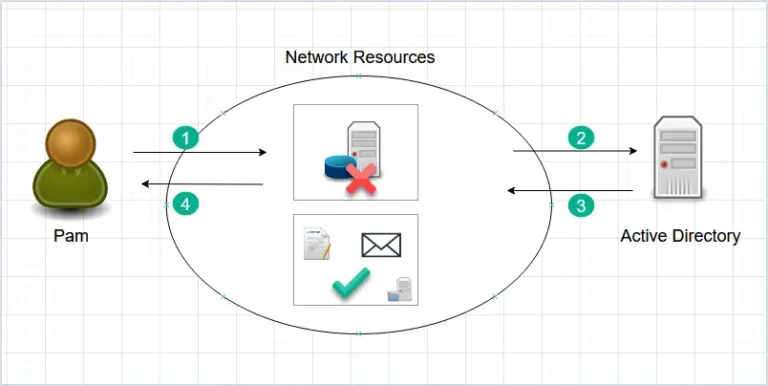
\includegraphics[width=0.75\linewidth]{auth2.png}
    \caption{Enter Caption}
    \label{fig:placeholder}
\end{figure}
In all of the above examples, Active Directory works by providing authentication and authorization to users and network resources. No matter what technical jargon you hear, that is the core function of Active Directory.

It is important to note that these network resources must be configured to use Active Directory. The resources are typically joined to the Active Directory server (but not all systems require this). There is a lot of configuration and planning that goes into configuring an Active Directory server. Organizations typically have dedicated professionals to implement and manage these systems.

In the next lesson, I will go over some of the core components of an Active Directory server.

\section{Active Directory Domain Services (AD DS)}
Active Directory Domain Services is the main component of Active Directory.

AD DS can be broken down into three main functions.

Directory service – A directory service provides methods for storing data in a structured way that makes administration and access easy. For example, Active Directory stores information on users, computers, and groups.

Authentication Service – Authenticates network users

Authorization Service – Grants or denies network users access to network resources.
It is important to stop here and review these three terms. Don’t get confused with the following three terms, they all refer to Active Directory.

AD – This is just an abbreviation for Active Directory.

AD DS – This is a server that is running the Active Directory Domain Services role.
Domain Controller (DC) – This is also a server that runs the Active Directory Domain Service Role. A Domain Controller is the same thing as a server running AD DS.

When you install Active Directory, you will be installing the AD DS Role on a Windows server.

\begin{figure}
    \centering
    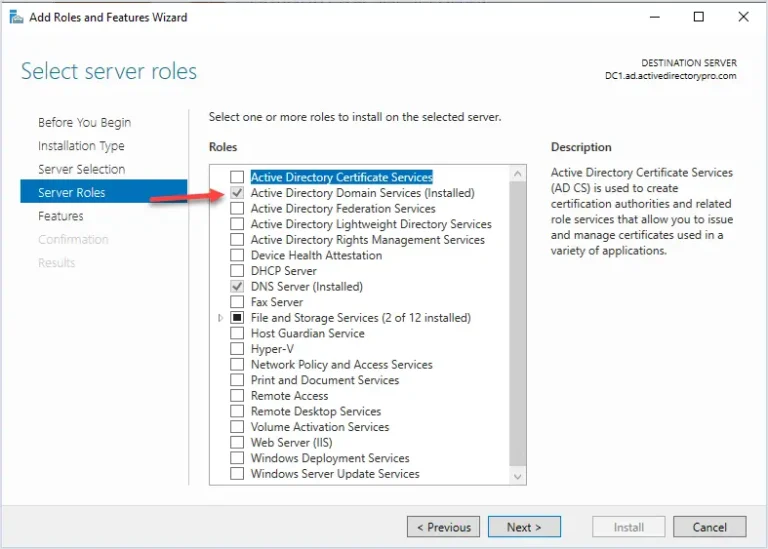
\includegraphics[width=0.75\linewidth]{dsrole.png}
    \caption{Enter Caption}
    \label{fig:placeholder}
\end{figure}

Next, we will go over some of the main components of AD DS.

\section{Active Directory Core Components}
You are about to see why Active Directory is a complex topic. I will briefly go over some of the core components of an Active Directory environment. I will include diagrams to help illustrate the topic. The components in the following are typical of any Active Directory environment.

\subsection{Active Directory Domains, Trees, and Forest}
Active Directory organizes resources in a hierarchical logical structure. This logical structure helps to organize objects, define relationships, and control security boundaries.

The forest is the top-level container and is a collection of Active Directory domains. The domains in the forest share a directory schema, a directory configuration, and a global catalog. Domains in the same forest automatically have a two-way transitive trust. When you first install Active Directory and create a domain, you are also creating a forest.

Active Directory Root Domain is a logical structure of containers and objects within Active Directory. A domain contains the following components:
\begin{itemize}
    \item Hierarchical structure for users, groups, computers, and other objects.
    \item Security services that provide authentication and authorization to resources in the domain and other domains
    \item Policies that are applied to users and computers
\end{itemize}

A DNS name to identify the domain. When you log into a computer that is part of a domain, you log into the DNS domain name. My DNS domain is \texttt{ad.hackherway.com}, this is how my domain is identified. 

When you install Active Directory, you have to pick a domain name to use. It is recommended to use a subdomain of a routable domain name. For example, \texttt{ ads.hackherway.com} is a subdomain of \texttt{hackherway.com}-this is the \textit{ top-level domain (TLD).} The initial installation of Active Directory creates a forest and a root domain.

The \textit{Child Domain} is a domain that shares the same domain name space as the root domain. It is a domain with its own collection of objects. In this example, there are two child domains \texttt{east.ad.hackherway.com} and \texttt{est.ad.hackherway.com.}

Trees are a set of domains that are connected together. When you add a child domain to a parent domain, you create what is called a \textit{domain tree}. A domain tree is just a series of domains connected together in a hierarchical fashion, all using the same DNS namespace. In the above diagram, the child domains \texttt{east.ad.hackherway.com} and \texttt{est.ad.hackherway.com} are part of the same domain tree.

\subsection{The Schema}
The Schema is a set of rules that defines the classes of objects and attributes contained in the directory.

\subsection{Global catalog (GC)}
A global catalog contains information about every object in the directory. This allows users and administrators to find the information in the directory regardless of which domain in the directory actually contains the data. By default, the first domain controller in a domain is designated as the GC server, it is recommended to have at least one GC server for each site to improve performance.

\subsection{Replication}
The replication service synchronized the Active Directory database with other domain controllers. Active Directory is typically deployed with two or more domain controllers for redundancy reasons. When you create an account on one Domain controller it is replicated to the other one. If one domain controller goes down, the other one will have a copy of the database.

\begin{figure}
    \centering
    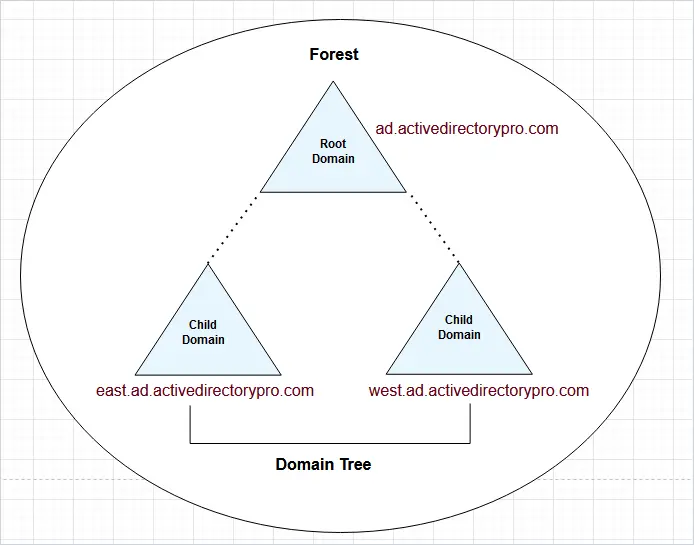
\includegraphics[width=0.75\linewidth]{treesforest.png}
    \caption{Enter Caption}
    \label{fig:placeholder}
\end{figure}

In the above diagram, if a user is added to DC1, it will be copied to DC2 and vice versa.

Active Directory sites for Sites and Services are used to combine multiple domain controllers into logical containers that relate to their physical location. Sites are used to optimize the performance of Active Directory when you have multiple branch offices and domain controllers.

\begin{figure}
    \centering
    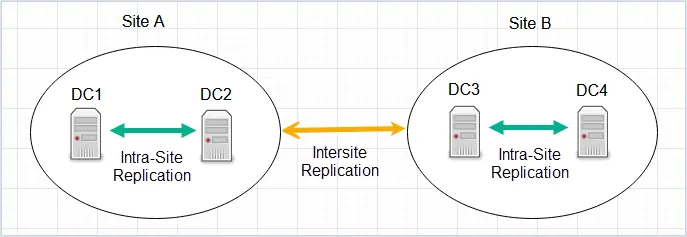
\includegraphics[width=0.75\linewidth]{intersiterepl.png}
    \caption{Enter Caption}
    \label{fig:placeholder}
\end{figure}

The above example has two sites, and each site has two domain controllers. The domain controllers in Site A use intrasite replication to keep all changes synchronized between DC1 and DC2. Site A and Site B use intersite replication to ensure that changes in Site A are replicated in Site B and vice versa.

\section{Kerberos}
Kerberos is the authentication protocol used by Active Directory to verify the identity of a user or host. The diagrams at the beginning of this guide looked simple, but in the background there was a lot of communication between the client and the Active Directory server to authenticate and authorize the user.

Here is a diagram showing the authentication process that takes place in the background.

\begin{figure}
    \centering
    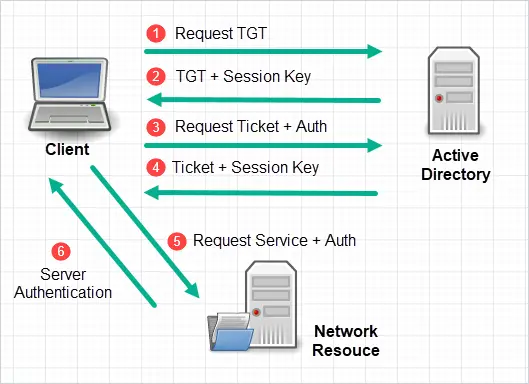
\includegraphics[width=0.75\linewidth]{kerbauth.png}
    \caption{Enter Caption}
    \label{fig:placeholder}
\end{figure}

\begin{enumerate}
    \item The client sends a request to the Active Directory server.
    \item The server responds with a TGT and session key that the client can use to encrypt and authenticate with the AD server.
    \item The client sends a request for a ticket.
    \item The server validates the request and returns a service ticket.
    \item The client uses the ticket received from the AD server to request access to a network resource.
    \item The server will decrypt the ticket and validate the request.
\end{enumerate}

\section{FSMO Roles}
Microsoft introduced \textit{Flexible Single Master Operation (FSMO)} roles in 2003. These FSMO roles can be distributed to different domain controllers, which can help with performance and redundancy. If one domain controller goes down, another DC will take over the missing role.

The \textit{Schema Master role} manages the read-write copy of the schema in Active Directory.

The \textit{Domain Naming Master role} makes sure that you do not create a second domain with the same name in a forest.

\textit{The RID master} is in charge of the SID for each object. Each AD object must have a unique SID. To prevent duplicates, the RID is in charge.

\textit{The PDC (Primary Domain Controller) Emulator} is the authoritative DC in the domain. It is responsible for authentication requests, password changes, and group policies.

The \textit{Infrastructure Master role} manages the relationship of GUIDS, SIDs, and DN between domains.

\begin{figure}
    \centering
    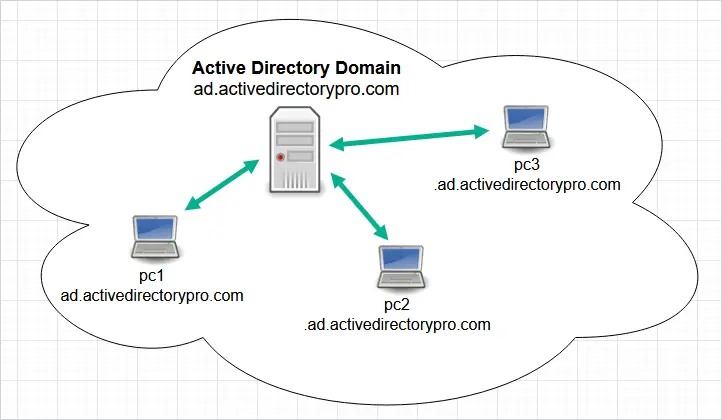
\includegraphics[width=0.75\linewidth]{addom.png}
    \caption{Enter Caption}
    \label{fig:placeholder}
\end{figure}

When you install Active Directory, you have to pick a domain name to use. It is recommended to use a subdomain of a routable domain name. For example, \texttt{ ads.hackherway.com} is a subdomain of \texttt{hackherway.com}

When you join a computer to the domain, it will have the DNS suffix of your domain name, for example, \texttt{pc1.ad.hackherway.com.}

This way, all of your domain joined systems are part of the same DNS namespace and can easily communicate with each other.

Also known as domain-joint, Active Directory domain, or Active Directory environment.

Windows Domain simply means your active directory server and its domain joined devices or systems using it for authentication and authorization.

User accounts
User accounts are used to provide employees access to network resources. A user account is typically assigned to each employee, but sometimes shared accounts are used. This account is stored in the Active Directory database and can provide details on the employee such as first name, last name, street, state, city, manager, etc.

Screenshot of a user account object in Active Directory.

\begin{figure}
    \centering
    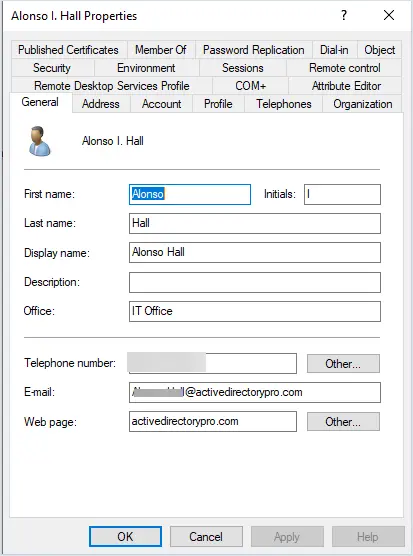
\includegraphics[width=0.75\linewidth]{aduser.png}
    \caption{Enter Caption}
    \label{fig:placeholder}
\end{figure}

Security Groups
A security group is a collection of users or computers. It simplifies the administration of permissions for a group of objects. For example, if 20 people need access to a file, you can create a security group and add the 20 people to the group. Then you would only have to manage file access for the group instead of 20 individual accounts.

Screenshot of a security group.

\begin{figure}
    \centering
    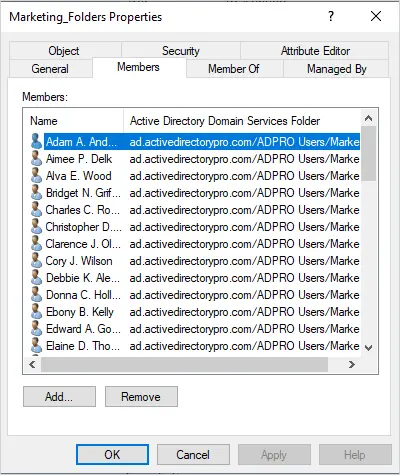
\includegraphics[width=0.75\linewidth]{usrgrp.png}
    \caption{Enter Caption}
    \label{fig:placeholder}
\end{figure}

Computers Objects
When a computer is joined to the Active Directory domain, a computer object is created. When the object is created in Active Directory, it becomes a trusted object which can be used to gain access to the network. For example, a user needs to log into the network and access a secured file. The user can log into the computer that is trusted and access the secured file (if the user has been granted access).

Screenshot of a computer object.

\begin{figure}
    \centering
    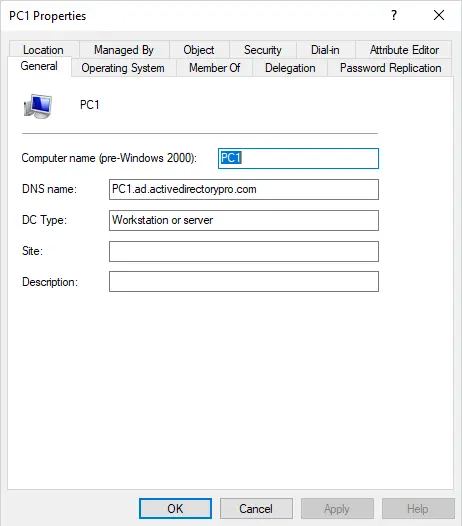
\includegraphics[width=0.75\linewidth]{compobj.png}
    \caption{Enter Caption}
    \label{fig:placeholder}
\end{figure}

Organizational Units (OU)
In Active Directory, organizational units are used to organize Active Directory Objects (users, groups, computers). Organizing your AD objects makes it easier to administrate and apply policies. For example, you could organize all users into their own department folders. It is recommended to separate users and computers into their own OU.

\begin{figure}
    \centering
    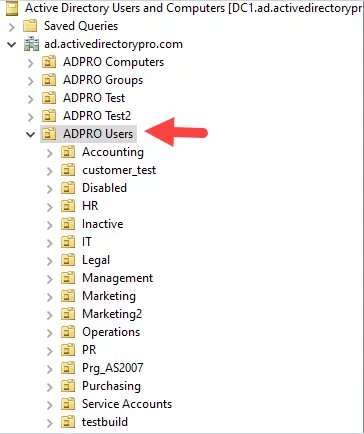
\includegraphics[width=0.75\linewidth]{OU.png}
    \caption{Enter Caption}
    \label{fig:placeholder}
\end{figure}

\section{Active Directory Benefits}
The main benefit of Active Directory is its ability to centralize user management and access to network resources.

Active Directory centralizes the management of the following:

Centralized management of user accounts
Centralized management of permissions
Centralized management of policy settings
Let us look at each of these benefits with some examples.

Benefit #1. Centralized Management of User Accounts
By using Active Directory, you have a single place to create and manage all user accounts.

For example, I will pretend Active Directory Pro has 100 employees and they all need the ability to access the network. An Administrator would use the Active Directory users and computer console and create all the accounts in one central location.

\begin{figure}
    \centering
    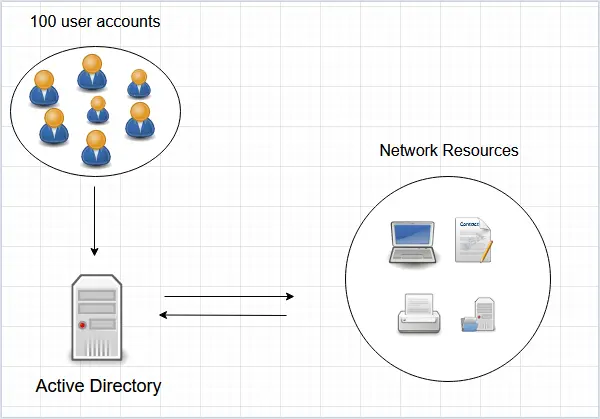
\includegraphics[width=0.75\linewidth]{centralaccts.png}
    \caption{Enter Caption}
    \label{fig:placeholder}
\end{figure}

The employees can now log into a computer and access all the resources they have access to.

Without an Active Directory, you would have to log into each resource and create an account. This would be a nightmare to manage and would be very time-consuming.

Here is what it would look like without an Active Directory server.

If Jim wanted to access network resources, an administrator would have to create the account on each system to which he needs access. For example, an account needs to be created on the laptop, on the database server, on the file server, on the email server, etc. Now you need to do that for 99 more employees. That would be a great pain.

This would be very time-consuming and impossible to create consistency across all users and resources.

\begin{figure}
    \centering
    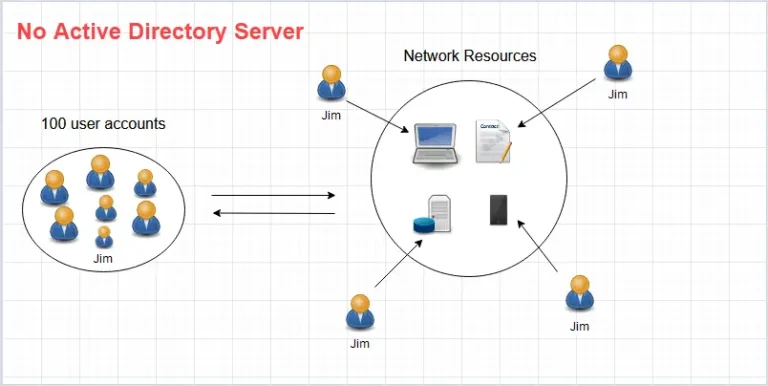
\includegraphics[width=0.75\linewidth]{noad.png}
    \caption{Enter Caption}
    \label{fig:placeholder}
\end{figure}

Benefit #2. Centralized Management of Permissions
By using Active Directory, you can centralize the control and management of permissions to your network resources.

Active Directory has security groups that can be used to give a group of user accounts access to resources.

For example, you have several users that need access to the accounting resources (server, contract file, file share). To easily provide access to all of these resources, you would add the users into an Active Directory security group that has permissions to these resources.

\begin{figure}
    \centering
    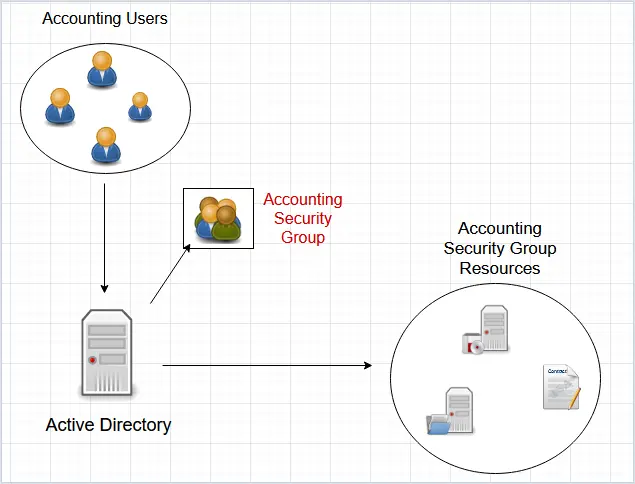
\includegraphics[width=0.75\linewidth]{perms.png}
    \caption{Enter Caption}
    \label{fig:placeholder}
\end{figure}

By using Active Directory security groups, you can easily grant and remove permissions. When an employee leaves or needs permissions removed, you just remove the account from the group.

Benefit #3 Centralized Management of Policy Settings
In an Active Directory environment, you can use group policy to apply policy settings to users and computers.

For example, if you want all users to change their password every 60 days, you can configure a password policy that applies to all users. If you wanted to apply power settings to all computers, you can do that with g\Group Policy.

\begin{figure}
    \centering
    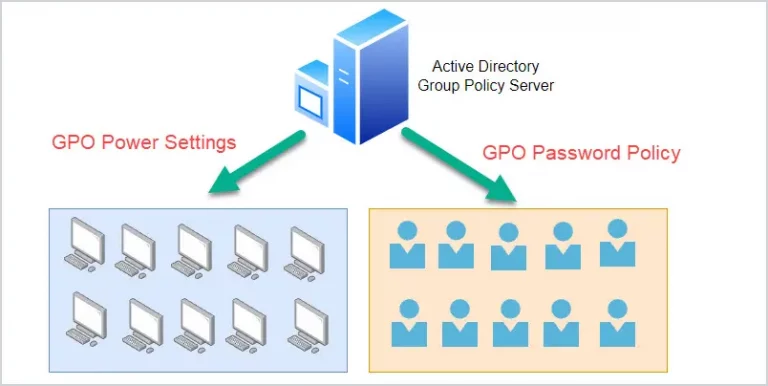
\includegraphics[width=0.75\linewidth]{gp.png}
    \caption{Enter Caption}
    \label{fig:placeholder}
\end{figure}

With no Active Directory or group policy, you would need to configure the policy settings on each computer. That would be impossible to manage in large environments. Organizations that are 100\% in the cloud use Microsoft Intune to manage policy settings. Intune can also be used in hybrid environments.

\section{Active Directory Management Tools}
In this lesson, you will learn about the various tools used to manage Active Directory. Most of these are included when you install Active Directory on a server.

On the server running Active Directory, you can access these management tools in the 'Windows Administrative Tools' folder. You can also install these tools on another computer by installing the RSAT tools.

\begin{figure}
    \centering
    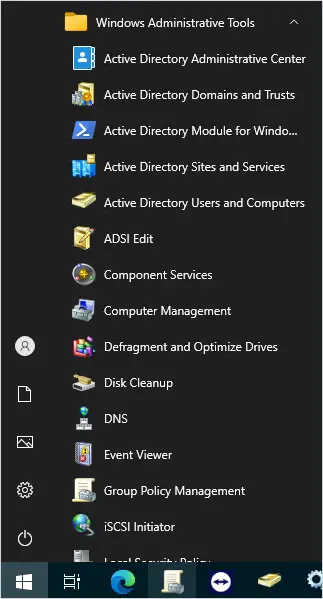
\includegraphics[width=0.75\linewidth]{rsat.png}
    \caption{Enter Caption}
    \label{fig:placeholder}
\end{figure}

Active Directory Users and Computers (ADUC)
This is the console that is used to create and manage user accounts, computers, and groups. For example, to create a new user account, you would open the ADUC console to create the new account, set the password, and add the user to groups. It is also used to create OUs and organize your objects.

\begin{figure}
    \centering
    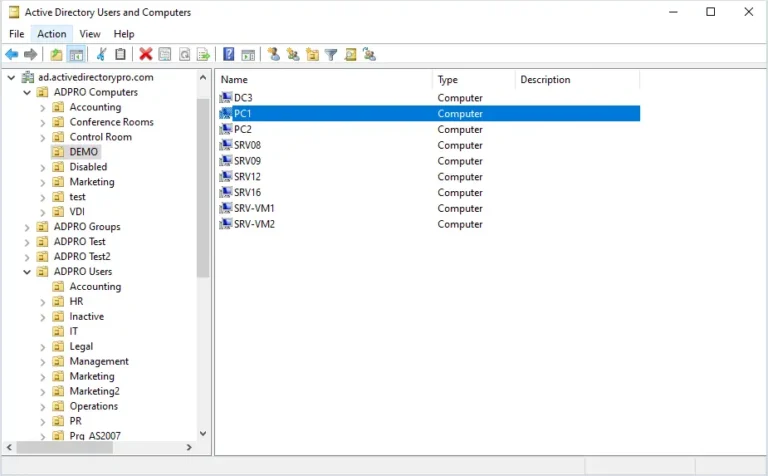
\includegraphics[width=0.75\linewidth]{aduc.png}
    \caption{Enter Caption}
    \label{fig:placeholder}
\end{figure}

Active Directory Administrator Center (ADAC)
The ADAC tool was included with server 2008 R2 and higher. It performs many of the same tasks as ADUC and a few additional ones. I’m not sure if Microsoft meant for this to replace ADAC but it is not widely used. Most administrators still use the ADUC tool.

\begin{figure}
    \centering
    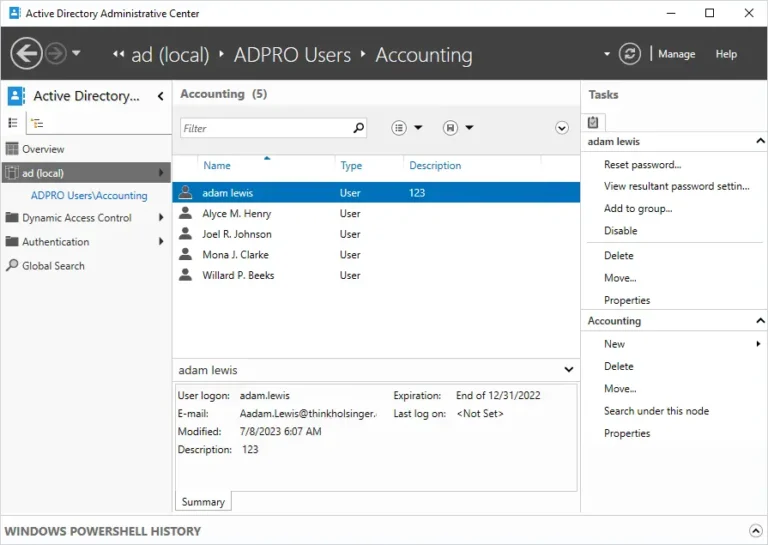
\includegraphics[width=0.75\linewidth]{adac.png}
    \caption{Enter Caption}
    \label{fig:placeholder}
\end{figure}

Active Directory Domains and Trusts
This console is used to raise the domain mode or functional level of a domain or forest. It is also used to manage trust relationships. This console is one that you will not use very often.

\begin{figure}
    \centering
    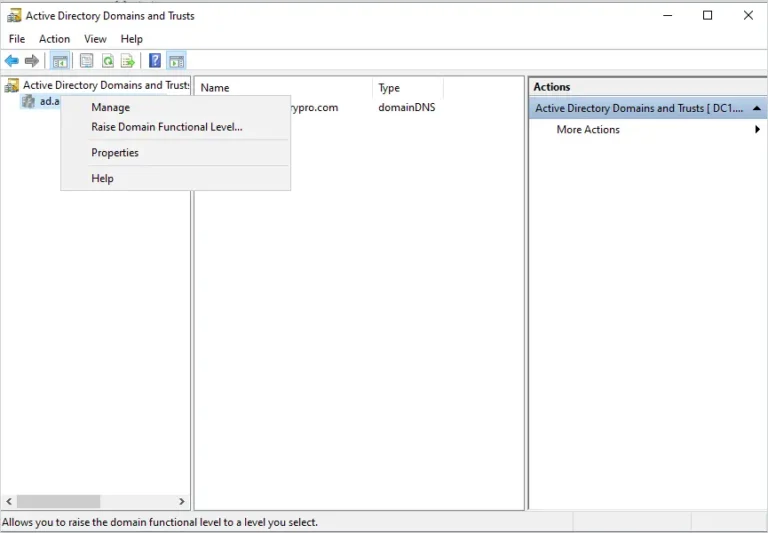
\includegraphics[width=0.75\linewidth]{domtrust.png}
    \caption{Enter Caption}
    \label{fig:placeholder}
\end{figure}

Active Directory Sites and Services
This console is used to manage your sites and subnets. If you only have a single site, then you will not need to use this console. If you deploy Active Directory in multiple geographic regions, you may need to use this console to manage your subnets, sites, and replication.

\begin{figure}
    \centering
    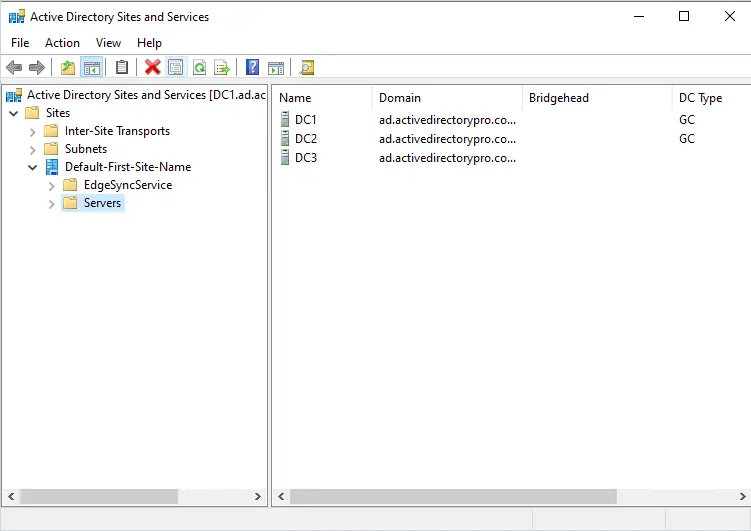
\includegraphics[width=0.75\linewidth]{adss.png}
    \caption{Enter Caption}
    \label{fig:placeholder}
\end{figure}

Group Policy Management Console
Group policy provides centralized management and policy settings for users and computers in an Active Directory environment. For example, to make sure all users change their password every 90 days, you would use group policy and configure a password policy. Understanding how to use group policy is a critical function as a System Administrator. 

\begin{figure}
    \centering
    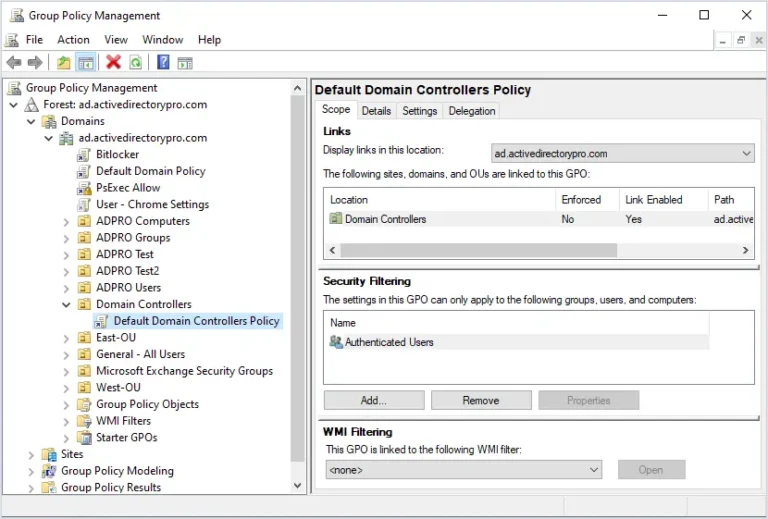
\includegraphics[width=0.75\linewidth]{gpm.png}
    \caption{Enter Caption}
    \label{fig:placeholder}
\end{figure}

DNS
The DNS console is used to manage and create DNS zones and resource records. Active Directory will not work without DNS; it is included when you install AD. It is important to know the basics of DNS if you are working with Active Directory.

\begin{figure}
    \centering
    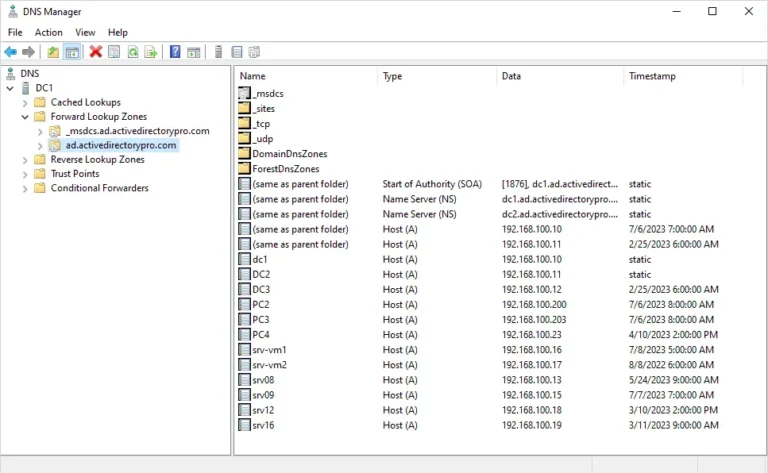
\includegraphics[width=0.75\linewidth]{dns.png}
    \caption{Enter Caption}
    \label{fig:placeholder}
\end{figure}

DHCP
The DNS console is used to create and manage the DHCP address pools in your network. This is one tool that actually has nothing to do with Active Directory. You don’t need DHCP for Active Directory, but it is typically used to simplify assigning IP addresses to client devices.

\begin{figure}
    \centering
    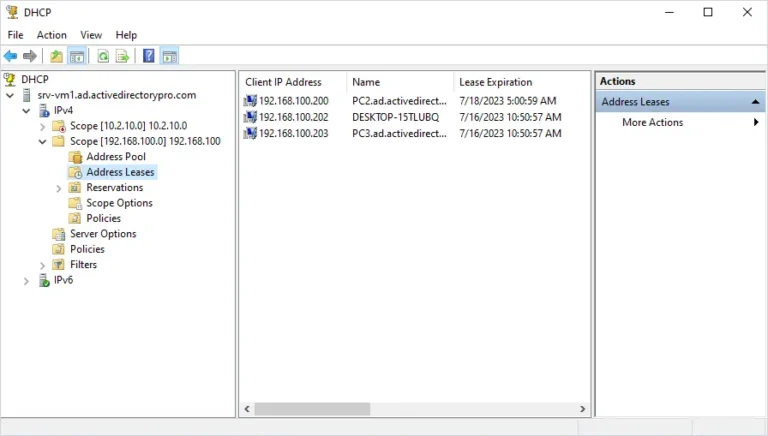
\includegraphics[width=0.75\linewidth]{dhcp.png}
    \caption{Enter Caption}
    \label{fig:placeholder}
\end{figure}

PowerShell
PowerShell is a command-line tool that helps you automate many routine tasks such as creating, updating, and reporting on objects in Active Directory.

Active Directory Pro Toolkit
The AD Pro Toolkit is a collection of Active Directory Management Tools used to simplify and automate the administration of Active Directory.

I have managed many Active Directory environments over my career as a System Administrator/Manager. The tools provided by Microsoft lack many features, such as bulk management and reporting. PowerShell can help with automation, but it can be time-consuming to figure out, and not all admins have this needed free time. That is why I created the toolkit, it is very easy to use and saves you a lot of time.

\begin{figure}
    \centering
    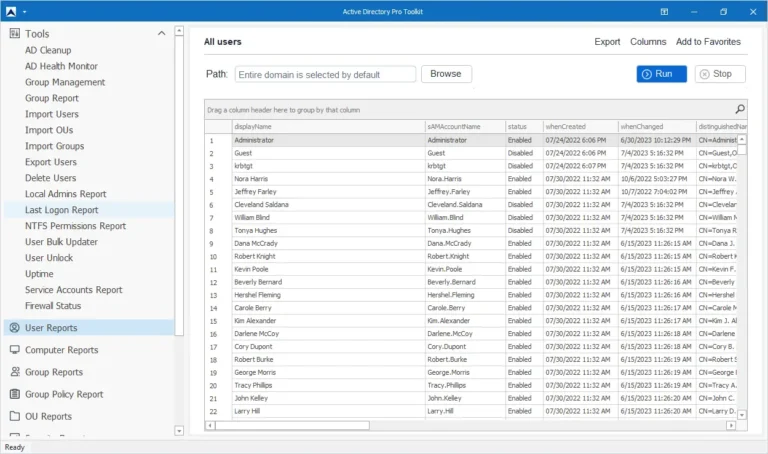
\includegraphics[width=0.75\linewidth]{adtoolkit.png}
    \caption{Enter Caption}
    \label{fig:placeholder}
\end{figure}

\section{Other Active Directory Services}
The following is a list of additional Active Directory services that can be installed. These services are optional and are installed by using the add roles and features wizard on the Windows server.

Active Directory Certificate Services
Certificate services are used to manage and deploy certificates. Certificates are used to digitally sign and encrypt documents and network traffic.

Active Directory Federation Services
The federation services provide single sign-on (SSO) for user accounts for web based applications such as Office 365.

Active Directory Lightweight Directory Services
AD LDS is a service that provides directory services for applications and also provides a data store and services for accessing the data store. It uses standard application programming interfaces (APIs) for accessing the application data.

Active Directory Rights Management Services
This service encrypts documents and is used to limit access to documents such as email, office documents, and Web pages.

\section{Azure Active Directory (AAD)}
Azure Active Directory is now called Entra ID.

Azure Active Directory (AD) is a cloud-based service for authenticating and authorizing access. Microsoft calls it an identity and access management service, which is a new fancy term that just means authenticate and authorize access.

Azure AD will authenticate users to cloud-based applications like Office 365, Azure, and other SaaS applications.

\begin{figure}
    \centering
    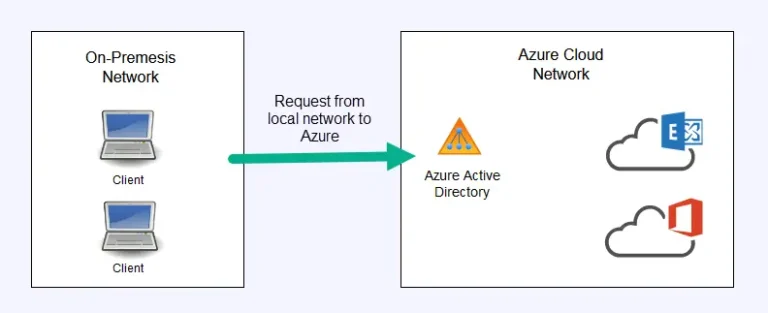
\includegraphics[width=0.75\linewidth]{aad.png}
    \caption{Enter Caption}
    \label{fig:placeholder}
\end{figure}

ADDS = Active Directory Domain Services (on-premises Active Directory).

AAD – Azure Active Directory (Cloud-based Active Directory).

Hybrid Azure AD
A hybrid Active Directory is when you have a local Active Directory (ADDS), and sync it with the cloud Azure Active Directory (AAD). In hybrid mode, you can sync your local AD with the Azure AD using a Microsoft software called Azure AD Connect. This enables you to have the same users and passwords on premises and in the cloud. This is done so that users will have a single sign on to both local resources and cloud-based resources.

\begin{figure}
    \centering
    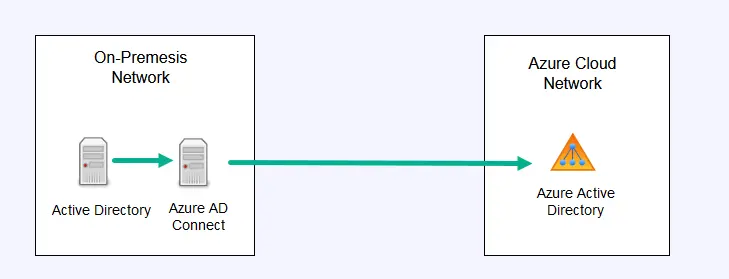
\includegraphics[width=0.75\linewidth]{aadcloud.png}
    \caption{Enter Caption}
    \label{fig:placeholder}
\end{figure}

The sync of local AD to cloud AD is a one-way sync, but Azure does not sync with the local AD.

What is Active Directory and why is it important?
In an organization, security is very important. It covers not only the physical setup of the company but also the security of their network. The general security of the organization’s network is a critical responsibility of the Network and System Administrator. Like people are filtered and screened as they enter the building, system administrators also need to make sure that only authorized users can access company resources. This is where Active Directory comes into the picture. 

Active Directory or AD plays a vital role in an organization. It is a form of database where users, groups, and computers are stored. Not only is it a database, but it also defines the security of the organization’s network. This would define who will have access to company resources, including what type of access they will have. As a result, only the defined users will have access according to their defined type of access. 

If you want to be a system administrator, your knowledge of Active Directory is very important. Let’s learn what an active directory is and how it plays a vital role in an organization and its components. 

What are the components of AD?
Now let us get into the details of the components of AD. In a Windows Server Operating System, AD is termed Active Directory Domain Services or AD DS. According to Microsoft, AD DS provides the methods for storing directory data and making these data available to network users and administrators. A window server running AD DS is called a domain controller. AD has four major components, domain, tree, forest, and objects.  

Domain, or Active Directory domain, is typically a collection of all objects within an AD DS network. This is grouped in a tree structure. AD domains are identified by a DNS name that is usually the same as the organization’s public domain name, subdomain, or any alternate version. 
Tree – is a collection of domains within AD DS. The main reason why it is called a tree is because each domain has exactly one parent, which leads to a hierarchical tree structure. A domain tree typically starts from a single parent or root and then branches out into different child domains.
Forest – this is considered the highest level of organization within AD. It also acts as the centralized mechanism for managing and controlling authentication and authorization across the organization. 
Object - refers to the single element contained in an AD such as a user, group, application, and devices. It may also be defined as resources or security principals.

\begin{figure}
    \centering
    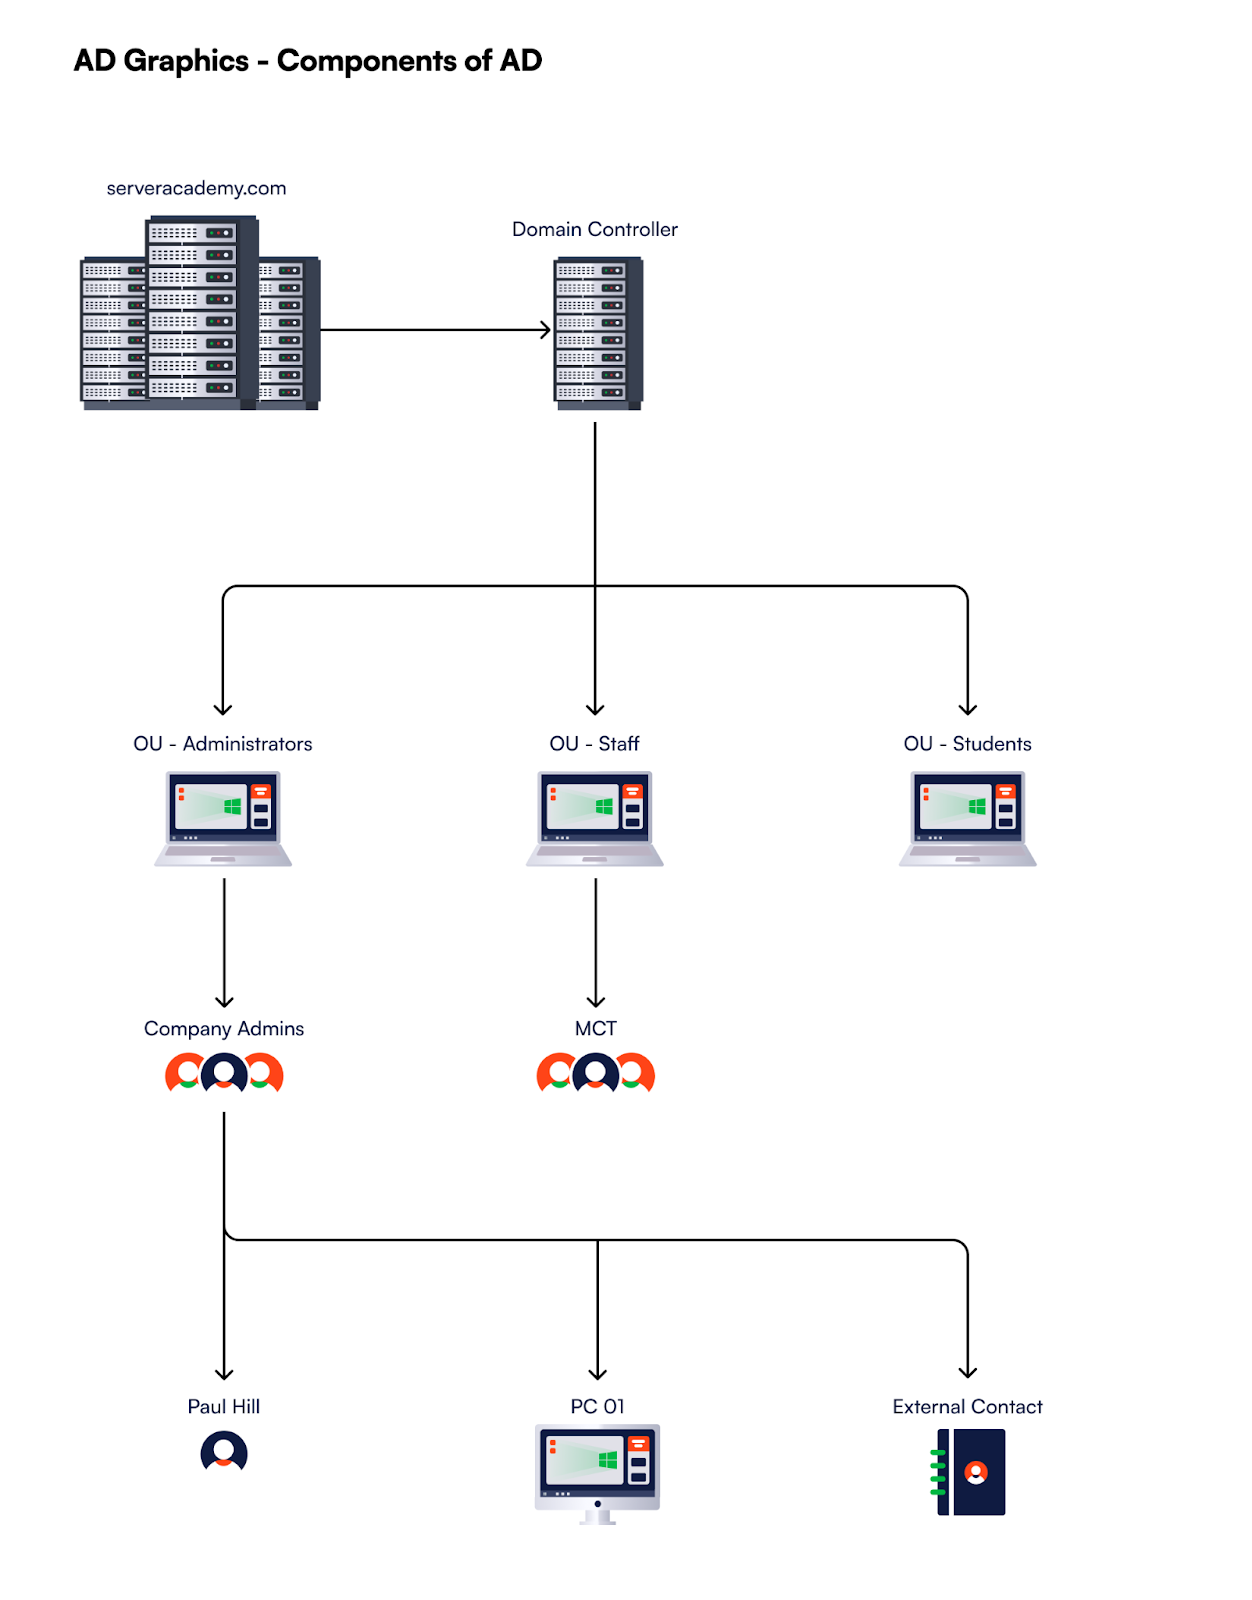
\includegraphics[width=0.75\linewidth]{adcomp.png}
    \caption{Enter Caption}
    \label{fig:placeholder}
\end{figure}

What are AD Objects?

As discussed above, Active Directory is composed of four major components and one of which is an Object. Listed below are the different types of objects that you need to be familiar with in order to administer Active Directory successfully:

User
Contact
Computer
Shared folder
Group
Organization Unit
Domain
Domain Controller
Site
Now that you know the different types of objects in Active Directory, let’s get into the details of each object.

User - This type of object represents a real user who is an active part of an organization’s AD network. A user object can be an employee of the organization such as IT Admins, Human Resources managers, Directors, and Executives who may usually have an elevated permission compared to other users.
Contact – similar to a user object, a contact in AD represents a real contact person who is not part of the organization. They may have a significant contribution or role in the organization such as partners, vendors, or agencies that have specific tasks or roles in the organization.
Group – this type of object can contain other AD objects such as other groups, users, as well as computers and printers. The group object serves as a container type of object in Active Directory.
Organizational Unit (OU) - Like group objects, organizational unit objects can also contain other AD objects.
Domain – this is a structural component of the active directory. Like group and OU objects, domains can contain other AD objects. Each domain in an AD has its own database and its own set of defined policies that are applied to all AD objects within it.
Domain Controller – this object is responsible for maintaining the policies, authentication to all AD users and provides roles that other Domain Controllers in a domain should be performing.
Site - This object in AD is overall in charge of managing and facilitating the process of replications.
Built-in - These objects contain local groups that are predefined during the creation of the active directory.
Apart from understanding the different types of AD objects, as a system administrator, it is also important that you understand the two main categories of AD objects, leaf and container AD objects.

Container AD Objects - These are objects that can contain other AD objects within them. A good example of this object is Organization Unit and Groups.
Leaf AD Objects - These are objects that cannot contain other objects within them such as User, Computer, and Printer.

\begin{figure}
    \centering
    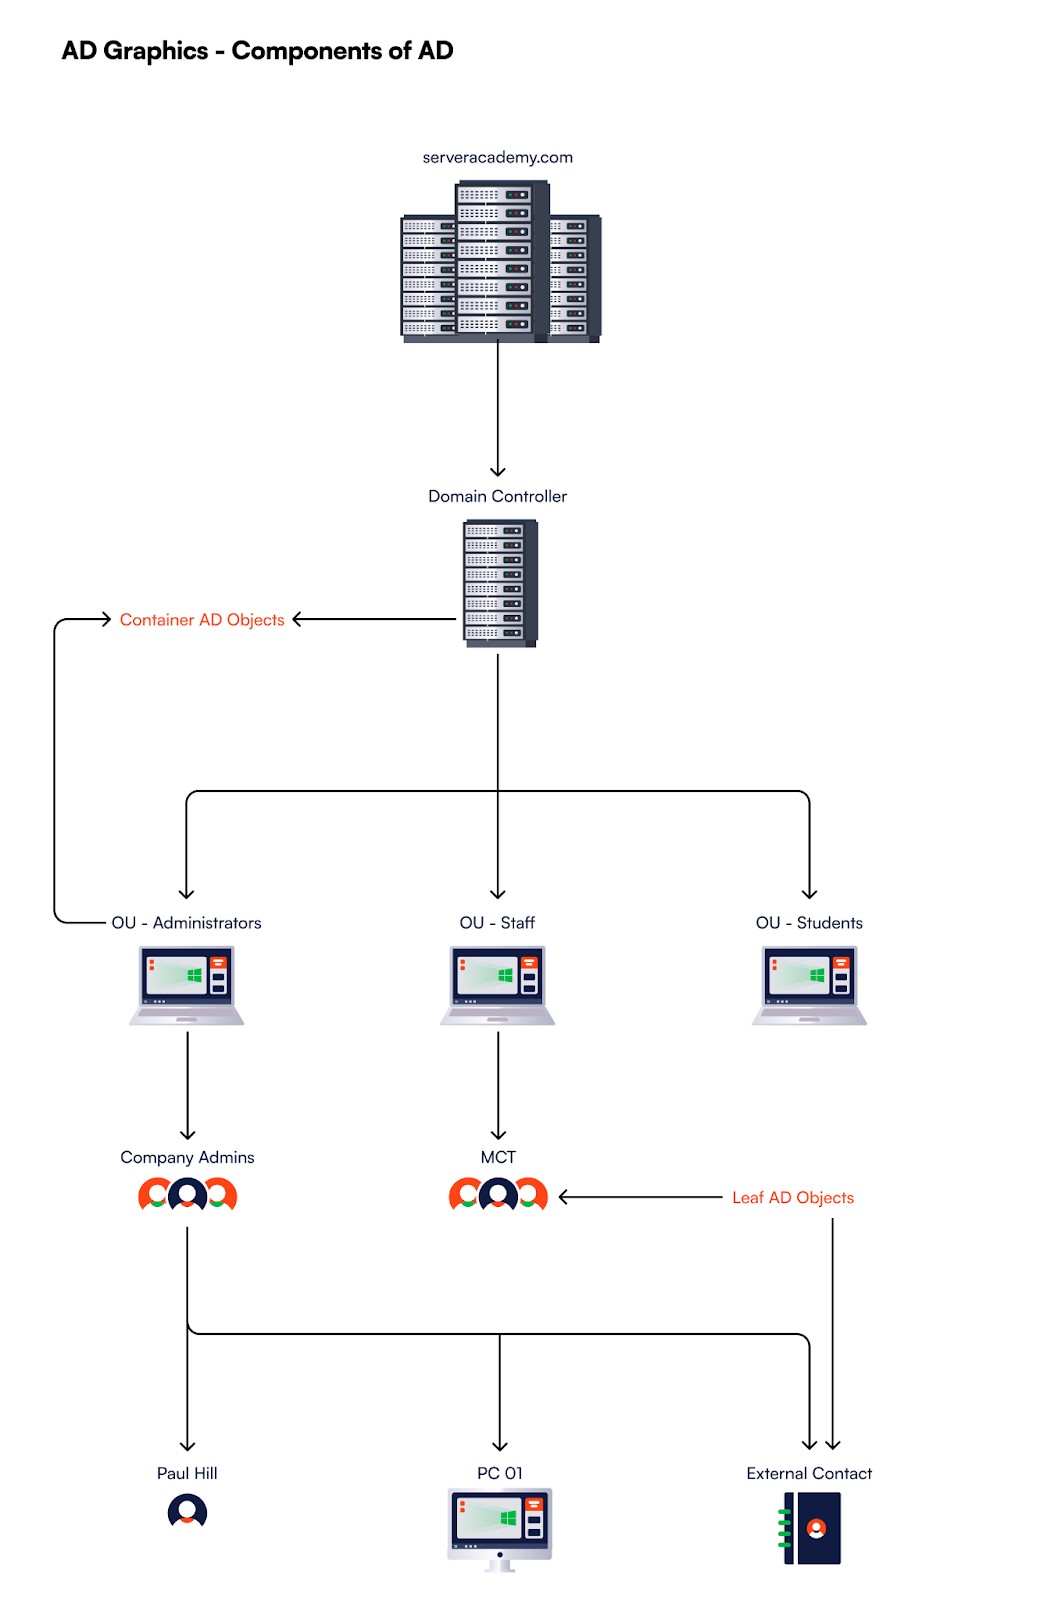
\includegraphics[width=0.75\linewidth]{adcomp2.png}
    \caption{Enter Caption}
    \label{fig:placeholder}
\end{figure}

Now that you know the components of an AD, let us also get into the details of a domain. As discussed above, a domain serves as the structural component of your organization. It serves as the fundamental unit of AD that typically shares common administration, security, and replication requirements. Active directory can have multiple subdomains. This is how a system administrator will design the AD if the organization has several regions of business or branches. 

\begin{figure}
    \centering
    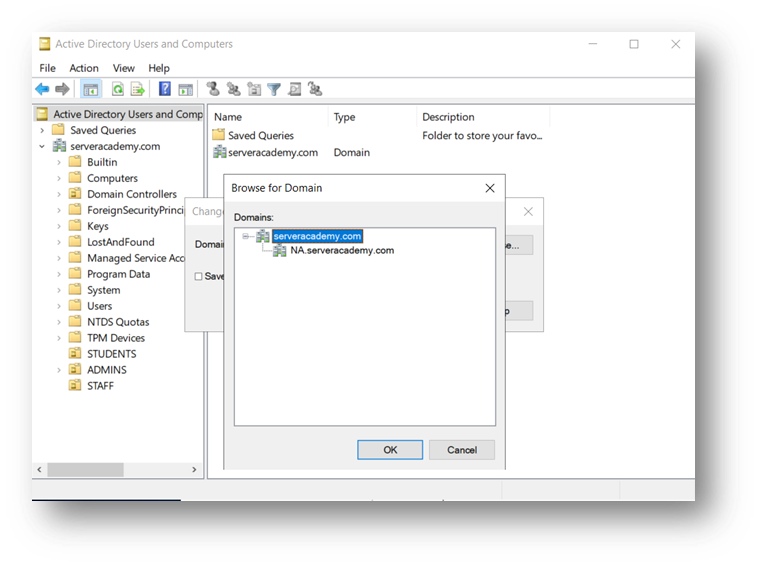
\includegraphics[width=0.75\linewidth]{aduc1.png}
    \caption{Enter Caption}
    \label{fig:placeholder}
\end{figure}

Subdomains on the other hand allows a logical partitioning of Active Directory. This fits perfectly if the organization has several regions of their business. You can divide active directory into smaller directories to allocate rights delegation to the subdomains. With this setup you will be able to keep everything organized from an administrative standpoint.

Your main goal as the system administrator is to build up the structure for your organization to support delegation of permission. This is also to take advantage of all customizations of policies without applying it to every single user or object in your active directory. Speaking of building up the structure, managing a large-scale organization would require some users to be able to access networks or resources from one location to another without issuing different credentials. For example, a company director should be able to login to a computer from the headquarters and to another computer located offshore. This is where Domain Trust comes in.

An Active Directory trust (AD trust) is a way of connecting two different or distinct AD domains or forests to allow users in one domain to be authenticated against resources from the other domain. This serves as a communication bridge that establishes the connection of one domain and another domain in your organization’s AD network. With this connection, resources between two different domains can be shared, and therefore provide seamless access to the users. 

Another term you would hear a lot is Domain Controller. It is a windows server that manages network, identity, security, and policies and hosts the Active Directory database. It effectively acts as a gatekeeper for the authentication and authorization of users into your organization’s IT resources within the domain. Therefore, it is very important to secure the domain controller. It serves as the key door in your organization’s IT resources. If you want to learn how to start creating your own active directory domain, click here. 

As a system administrator, you may also encounter some unexpected failures in managing the active directory. Some or maybe the whole network or system may fail to access company resources because of this. There are also instances that your network administrator depends on Active Directory to assign IP addresses to all of your company devices via DHCP server or DNS server which are both being managed under your domain controller. As critical as this set up, it is important to have multiple domain controllers for replication and redundancy. 

AD allows the possibility of maintaining a writable copy of its own domain partition. To put it simply, it replicates automatically whatever changes are made to your domain controller to your other domain controllers. This process is called multimaster replication. This allows most of the operations to be processed reliably by multiple domain controllers, and so it provides high levels of redundancy, availability, and accessibility in your Active Directory. With all of these capabilities, you have to apply some exceptions to some AD operations that are highly sensitive, or simply restrict them to a specific domain controller. This is where the Flexible Single-Master Operator (FSMO) roles. 

Before we discuss these five roles, let us give you an overview of how FSMO roles work. In every forest, there is a single Schema Master and a single Domain Naming Master. In each domain, there is one Infrastructure Master, one RID Master, and one PDC Emulator; however, at any given time, there can be only one DC performing the functions of each role. Therefore, a single DC could run all five FSMO roles; however, in a single-domain environment, there can be no more than five servers that run the roles.

\begin{figure}
    \centering
    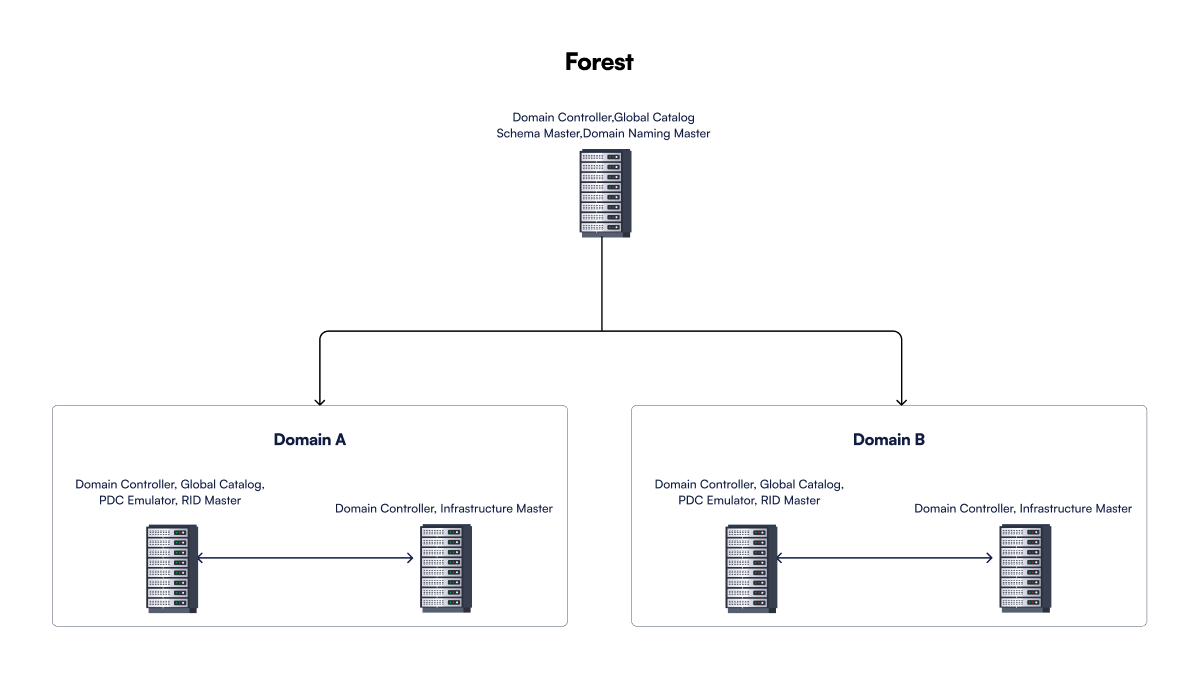
\includegraphics[width=0.75\linewidth]{adforest.png}
    \caption{Enter Caption}
    \label{fig:placeholder}
\end{figure}

An Active Directory has five FSMO roles:

Schema Master – Schema Master is an enterprise-level FSMO role; There is only one Schema Master in an Active Directory forest. The Schema Master role owner is the only domain controller in an Active Directory forest that contains a writable schema partition. As a result, the DC that owns the FSMO Master Schema role must be available to modify its forest schema. Examples of actions that update the schema include raising the functional level of the forest and upgrading the operating system of a DC to a higher version than currently exists in the forest. 
Domain Naming Master – Domain Naming Master is an enterprise-level role; there is only one Domain Naming Master in an Active Directory forest. The Domain Naming Master role owner is the only domain controller in an Active Directory forest that is capable of adding new domains and application partitions to the forest. Its availability is also necessary to remove existing domains and application partitions from the forest. The Domain Naming Master role has little overhead, and its loss can be expected to result in little to no operational impact, since the addition and removal of domains and partitions are performed infrequently and are rarely time-critical operations. Consequently, the Domain Naming Master role should need to be seized only when the DC that owns the role cannot be brought back online.
Infrastructure Master – Infrastructure Master is a domain-level role; there is an Infrastructure Master in each domain in an Active Directory forest. The Infrastructure Master synchronizes objects with the global catalog servers. The Infrastructure Master will compare its data to the data of a global catalog server and receive any data not found in its database from the global catalog server. If all DCs in a domain are also global catalog servers, then all DCs will have up-to-date information (assuming that replication is functional). In such a scenario, the location of the Infrastructure Master role is irrelevant, since it does not have any real work to do.
Relative ID (RID) Master – Relative Identifier Master (RID Master) is a domain-level role; there is one RID Master in each domain in an Active Directory forest. The RID Master role owner is responsible for allocating active and standby Relative Identifier (RID) pools to DCs in its domain. RID pools consist of a unique contiguous range of RIDs, which are used during the creation of the object to generate the unique Security Identifier (SID) of the new object. The RID Master is also responsible for moving objects from one domain to another within a forest.
PDC Emulator – The Primary Domain Controller Emulator (PDC Emulator or PDCE) is a domain-level role; there is one PDCE in each domain in an Active Directory forest. The PDC Emulator controls the authentication within a domain, whether Kerberos v5 or NTLM. When a user changes their password, the change is processed by the PDC Emulator.
What are the duties of an Active Directory administrator?

An Active Directory administrator plays a critical role not just in the IT department but also in the entire organization. You are in charge of one of the most precious resources of any company, data. Some of your primary duties will include:

Creating and maintaining user accounts, schema, and groups
Controlling the domain and ensuring overall system security
Establishing and implementing group policies
Offering technical assistance to users
Ensuring compliance to policies and regulations
Helping with disaster recovery
Performing security audits

\section{Key Roles for Defenders in Active Directory}
A defender's security stance, or role, in Active Directory is responsible for protecting the AD environment from cyberattacks through proactive measures, continuous monitoring, threat detection, and incident response. Because AD is a primary target for attackers seeking credentials and access to corporate resources, a defender's role is a cornerstone of an organization's entire cybersecurity stance.

An Active Directory defender has key defensive responsibilities, such as (but not limited to):
\subsubsection{Preventative Measures and Hardening}
\textbf{Implement the Principle of Least Privilege (PoLP):}
Minimize the number of privileged accounts, including Domain Admins, and use Role-Based Access Control (RBAC) to grant users only the permissions necessary for their job roles and functions.

\subsubsection{Enforce Strong Password Policies and MFA:}
Mandate the use of long, complex passwords or passphrases and enforce MFA for all privileged accounts to prevent credential theft and brute-force attacks.

\subsubsectionSecure Administrative Access:}
Secure administrative access: Require administrators to use separate, nonprivileged accounts for daily tasks and access AD only from dedicated, hardened workstations (SAWs).

Protect Domain Controllers (DCs): Isolate DCs with network segmentation, restrict physical access, enforce strong firewalls, and periodically patch and update their operating systems.
Manage accounts and groups: Regularly audit and remove inactive or unused accounts that could serve as backdoors for attackers. Properly manage service accounts, using Group Managed Service Accounts (gMSA) when possible. 
Detection and monitoring
Continuous monitoring and auditing: Use Security Information and Event Management (SIEM) tools to centrally collect and analyze AD security logs in real-time. This helps detect suspicious activities, such as
Spikes in failed login attempts.
Changes in highly privileged security groups.
Unauthorized changes to Group Policy Objects (GPOs).
Leverage threat detection tools: Employ solutions that use advanced analytics and behavioral monitoring to identify more sophisticated attack techniques that may not be logged, such as DCShadow and Kerberoasting. 
Incident Response and Recovery Threat Containment: In the event of a breach, quickly contain the attack by isolating compromised systems, enabling accounts, and revocation of unauthorized access rights.
Forensics and investigation: Conduct a thorough investigation to determine how the breach occurred, what assets were affected, and how the attacker moved through the network. Detailed archived logs are crucial for this process.
Recovery and remediation: Restore AD from clean, offline backups to ensure the integrity of the environment. Remediate any vulnerabilities discovered to prevent a recurrence of the attack.
Develop a disaster recovery plan: Establish and test a formal AD recovery plan that includes procedures for backup, recovery, and communication during a security incident. 
Who performs these defensive tasks?
While responsibilities can vary by organization, defensive security tasks for Active Directory are often a joint effort between several teams, including
IT Security: Typically, a security policy is set with "guardrails," defining standards for everything from password length to MFA requirements.
IT Administrators: Responsible for the daily implementation of security policies, such as creating user accounts and managing group memberships, while operating within the rules set by the security team.
Security Operations Center (SOC): A dedicated team focused on continuous monitoring, incident detection, and the initial stages of incident response.
Identity and Access Management (IAM): Manages identity and access policies, ensuring that security groups and access controls adhere to the Principle of Least Privilege.

\subsection{The Role of the Attacker (Offensive Security) in Active Directory}
In the context of Active Directory (AD), the offensive security role involves acting as a simulated adversary, or "red teamer," to proactively identify vulnerabilities and misconfigurations that a malicious attacker could exploit. Using the same tools, tactics, and techniques as real hackers, offensive security professionals help organizations strengthen their defenses before a breach occurs. 
Offensive tactics against Active Directory
Offensive security professionals conduct exercises to exploit weaknesses in AD and escalate privileges. The typical attack lifecycle against an AD environment includes:
1. Reconnaissance
Attackers begin by gathering information about the target network and its AD environment to find a foothold.
Enumerating Users and Groups Attackers query AD for user, group, and computer information, looking for privileged accounts and misconfigured permissions.
Scanning ports: Tools such as Nmap are used to identify running services like Kerberos (port 88) and LDAP (port 389), which indicate a domain controller.
Trust Enumeration: Attackers map trust relationships between different domains or forests, as a compromised domain could allow access to a more privileged one.
Using Reconnaissance Tools: Tools such as PowerView and BloodHound are commonly used to gather information and visually map potential attack paths. 
2. Initial access and credential theft
Once initial access is gained, the focus shifts to stealing credentials to move laterally and escalate privileges.
Password spraying: This technique tries some common passwords against many different user accounts to avoid triggering account lockouts.
Kerberoasting: Attackers target Service Principal Names (SPNs) to request service tickets, which are then cracked offline to find the associated service account's plaintext password.
LLMNR/NBT-NS poisoning: This man-in-the-middle (MITM) attack intercepts local network traffic to capture NTLM hashes, which can be cracked offline.
Pass-the-Hash/Ticket: After obtaining a user's password hash or Kerberos ticket, an attacker can reuse it to authenticate to other services or systems without knowing the plaintext password. 
3. Privilege escalation
With stolen credentials, attackers try to gain a higher level of access, often aiming for Domain Administrator privileges.
Exploiting Misconfigurations: AD environments are complex and subtle misconfigurations can lead to significant vulnerabilities. For example, a service account with domain administrator privileges is a high-value target.
Abusing ACLs and Delegation: Attackers analyze Access Control Lists (ACLs) to find overly permissive settings that allow a standard user to perform privileged actions, such as resetting an admin's password.
Golden Ticket attacks: If an attacker gains the hash of the KRBTGT account, they can forge Kerberos tickets to gain permanent, domain-wide administrative access.
Extracting NTDS.dit: The ntds.dit file contains all AD password hashes. If an attacker can extract this file from a domain controller, they can attempt to crack every user's password offline. 
4. Persistence and defense evasion
Once access is escalated, the attacker's goal is to maintain a foothold and avoid detection.
Creating backdoors: Attackers can create hidden backdoors, such as new admin accounts or malicious registry keys, to regain access later.
Maintaining persistence: Techniques like WMI Event Subscriptions can be used to execute malicious code with elevated privileges, ensuring the attacker's, 

access survives reboots and other changes.
Abusing trusts: Attackers can manipulate trust relationships to pivot between different domains or forests, extending the scope of the attack. 
Why this role is important for security
By simulating these attacks, offensive security professionals provide critical insights that help defensive "blue teams" prepare for and respond to real-world threats. The intelligence gathered from these exercises allows organizations to:
Validate security controls: Prove whether firewalls, EDR, and other security measures actually work.
Test incident response: Evaluate the security team's ability to detect, contain, and remediate a breach.
Reduce risk proactively: Identify and patch vulnerabilities before a malicious actor can exploit them.
Meet compliance standards: Demonstrate security readiness to satisfy industry regulations and compliance requirements and/or mandates.

\section{Active Directory Certificate Services (AD CS)}
Active Directory Certificate Services (AD CS) is Microsoft's PKI implementation that integrates with existing Active Directory forests;

AD CS is not installed by default; is responsible for:
User Authentication
HTTPS Certificates
SSL VPN Certificates
Digital Signatures
Code signing

\section{AD CS \& PKI}
The Public Key Cryptography for Initial Authentication in Kerberos (PKINIT) protocol enables the use of public key cryptography in the initial authentication exchange of the Kerberos authentication protocol.

Instead of sharing a secret key between the client and KDC, the client possesses a public key pair that is signed by a trusted Certification Authority (CA).

When PKINIT is enabled, it is possible to:
Perform Kerberos authentication using X.509 certificates and obtain a TGT
Create an Schannel Security Context using X.509 certificates for LDAP over SSL (LDAPS)
Recover NTLM from TGT requested using X.509 certificates (UnPAC-the-Hash)

\section{Authenticating with Certificates When PKINIT is Not Supported}
How to obtain domain admin privileges during internal assessments. 

Here is what usually happens when we conduct an internal penetration test on an environment that has not been hardened against AD CS attacks:

1. Obtain a domain account (e.g., through Responder or mitm6)
2. Find the AD CS web enrollment service (e.g., with a valid account and Certify / Certipy; or in black box through manual search, or \texttt{ntlmrelayx.py --dump-adcs} option)
3. Force a Domain Controller to connect back to our workstation (e.g., through \texttt{printerbug.py,} or PetitPotam
4. Relay this authentication to the AD CS Web enrollment service with \texttt{ntlmrelayx.py} (attack ESC8 to obtain a certificate for the targeted DC)
5. Use \texttt{PKINITtools} to get a TGT for the target DC (or recover its NT hash), allowing us to take over the domain.

\section{Abusing Active Directory Certification Services (AD CS)}
Active Directory Certificate Services has an enormous attack surface.
In June 2021, Will Schroeder and Lee Christensen from SpectreOps published a whitepaper titled \textit{"Certified Pre-Owned."} that demonstrates how any adversary can utilize and abuse the AD CS environment to elevate privileges, gain a toehold and establish persistence with the breached network.
\begin{quote}
    Of note, nearly every environment with AD CS that we've examined for domain escalation misconfigurations has been vulnerable. It is hard for us to overstate what a big deal these issues are." - SpectreOps Team
    \end{quote}
    
\textbf{User Credential Theft (1 year +)}
Stealing existing user certificates capable of domain authentication or actively requesting a new certificate from a user's context.
\textit{Survives user password changes and can be done without elevation or touching LSASS.}

\textbf{Machine Persistence (1 year +}
Stealing existing system certificates capable of domain authentication or actively requestion a new certificate from a systems'c ontext, combined with resource-based constrained delegation (or just S4U2Self).
\textit{Survives machine password changes and can be done without touching LSASS.}

\textbf{Domain Escalation Paths}
Misconfigured certificate templates that allow Subject Alternative Name (SAN) specification, vulnerable Certificate Request Agent templates; vulnerable template ACLs, the \texttt{EDITF_ATTRIBUTESUBJECTALTNAME2 flag being set; vulnerable CA permissions, or NTLM relay to web enrollment endpoints.

\textbf{Domain Persistence}
Stealing the Certificate Authority private key and forging Golden Certificates.

\subsection{Audit Certification Services}
To configure Certificate Services audit, you must enable "Audit Configuration Services" subcategory of advanced audit policy, and at the level of the CA server, additionally determine which event categories are to be logged.

It is recommended to select all events to audit.

Active Directory was first released with Windows Server 2000. Its primary function is to provide authentication and authorization to users on the network.

Authentication is the process where Active Directory verifies a user’s credentials (username and password). The user’s credentials are stored in the Active Directory database.
Authorization is the process that grants or denies a user to do something such as edit a file or access an application.
Since its release, Microsoft has added additional services to Active Directory, more on this in lesson 6. The topic of Active Directory can be very complex as there are many services and components that make it work. Just remember its core function is to authenticate and authorize users to network resources.

Even though there has been a big push to move everything to the cloud, Active Directory is still used by most medium and large organizations. A lot of organizations use Office 365 and cloud services and operate in a hybrid mode. This means the local Active Directory is synced with the cloud to provide seamless authentication to Office 365 resources such as email.

To better understand how Active Directory works let’s look at some examples. These examples provide a high-level overview of how Active Directory works.

Example 1 – Authenticate Users
Jim was recently hired as an accountant for Active Directory Pro. The IT administrator creates an account for Jim in Active Directory, the account is unique to Jim and contains details such as first name, last name, office, phone number, etc. Jim is provided with a username and password so he can log into the company’s network.

Jim logs into his laptop with the provided username and password.
The logon request goes to the Active Directory server to verify Jim’s username and password.
Active Directory looks up Jim’s account and verifies the username and password. The account has been verified.
Jim is now logged into his laptop and is authenticated to the domain.
authenticate active directory user
Example 2 – Authorize User (grant or deny permissions)
In this example, the Active Directory server will authorize access to network resources.

Jim logs into his computer using his username and password and wants to access his email, a contract file, and the accounting database server.
These network resources check with Active Directory to see if Jim’s account is authorized for access.
Active Directory verifies Jim’s account is authorized for access.
Jim’s account is granted access. Jim can now check email, modify the contract file and work on the database server.
authorize active directory user
Example 3 – Authorize and Deny User Access
In this last example, we will look at another user that has mixed access (allow and deny permissions.

Pam logs into the network with her username and password. She tries to access the same resources as Jim (email, a contract file, and a database server. )
These network resources check with Active Directory to see if Pam’s account is authorized for access.
Active Directory verifies Pam’s account (Authentication). AD also checks what resources Pam’s account has access to (Authorization).
Pam can now access email and the contract file but does not have permission to access the accounting database server.
deny user permissions
In all of the above examples, Active Directory works by providing authentication and authorization to users and network resources. No matter what technical jargon you hear, that is the core function of Active Directory.

It is important to note that these network resources must be configured to use Active Directory. The resources are typically joined to the Active Directory server (but not all systems require this). There is a lot of configuration and planning that goes into configuring an Active Directory server. Organizations typically have dedicated professionals to implement and manage these systems.

In the next lesson, I’ll go over some of the core components of an Active Directory server.

